% The short baseline neutrino detector
\section{Neutrino oscillations and anomalies in the observations}

Neutrino oscillations have been observed by numerous experiments, yet there's a discrepance in the results of the different experiments.
It is important to know how neutrino oscillations are modeled and the possible effects that alter our expected observations.
This section includes simple oscilation models, matter effects and results from the neutrino oscillation experiments \gls{lsnd} and MiniBooNE.

\subsection{Neutrino oscillation models}

Neutrino oscillations are a consequence of flavour neutrino mixing\marginnote{\ldots or lepton mixing} in vacuum\cite{Agashe:2014kda}.
This can be modeled using a linear combination of the fields of the massive neutrinos $\nu_m$ for the flavor neutrino field $\nu_f$ in the charged current weak interaction
\begin{equation*}
  \nu_f = \sum_m U_{fm}\nu_m,
\end{equation*}
where $f \in \{e, \mu, \tau\}$ is the index for the flavor eigentstate and $m \in \{1, 2, 3\}$ is the index for the mass eigenstate.

$U_{fm}$ is an unitary matrix generally called \emph{mixing} matrix\marginnote{\ldots but also known as the Pontecorvo-Maki-Nakagawa-Sakata (PMNS) mixing matrix}.
The parametrization of this unitary matrix depends on the number of neutrino flavors and their characterization into \emph{Majorana} or \emph{Dirac} particles\marginnote{Whilst Majorana particles are their own anti-particles, particle and anti-particle differ when dealing with Dirac particles.}.
Assuming there are $n$ neutrino flavors and $n$ massive neutrinos, the mixing matrix $U$ can be parametrized by $\frac{n(n-1)}{2}$ Euler angles (see figure \ref{fig:euler_angles}) and $\frac{n(n+1)}{2}$ phases in the case of Majorana neutrinos or $\frac{(n-1)(n-2)}{2}$ phases if neutrinos are Dirac particles\cite{Xing:2013woa}.

In the following 3 types of flavor field and mass field eigenstates are assumed.
We impose furthermore, that none of the eigenstates is identical to another
\begin{align*}
  \braket{\nu_{l'}}{\nu_l}             = \delta_{l'l}, \quad
  \braket{\bar{\nu}_{l'}}{\bar{\nu}_l} = \delta_{l'l}, \quad
  \braket{\bar{\nu}_{l'}}{\nu_l}       = 0,
\end{align*}
where $l \in \{e, \mu, \tau\}$ or $l \in \{1, 2, 3\}$.

In the case of Dirac massive neutrinos the representation of $U$ is given the three angles $\theta_{12}, \theta_{13}, \theta_{23}$ and just one \gls{cp} violation phase $\delta$
\begin{marginfigure}
  \centering
  \vspace*{1em}
  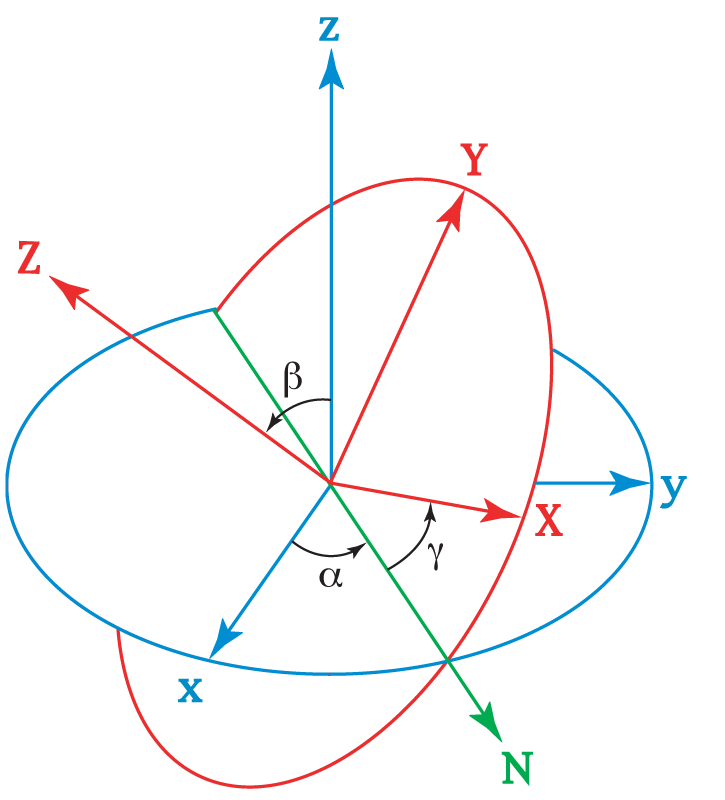
\includegraphics[width=\textwidth]{eulerangles}
  \caption{Illustration of the Euler angles between two rotated 3 dimensional reference frames.
  -- \copyright \href{https://commons.wikimedia.org/wiki/File:Euler.png}{wikimedia.org}}
  \label{fig:euler_angles}
\end{marginfigure}
\begin{align*}
  U_D &= \begin{bmatrix}
      U_{e 1} & U_{e 2} & U_{e 3} \\
      U_{\mu 1} & U_{\mu 2} & U_{\mu 3} \\
      U_{\tau 1} & U_{\tau 2} & U_{\tau 3}
    \end{bmatrix} \\
    &= \begin{bmatrix}
      1 & 0 & 0 \\
      0 & c_{23} & s_{23} \\
      0 & -s_{23} & c_{23}
    \end{bmatrix} \begin{bmatrix}
      c_{13} & 0 & s_{13}e^{-i\delta} \\
      0 & 1 & 0 \\
      -s_{13}e^{i\delta} & 0 & c_{13}
    \end{bmatrix} \begin{bmatrix}
      c_{12} & s_{12} & 0 \\
      -s_{12} & c_{12} & 0 \\
      0 & 0 & 1
    \end{bmatrix} \\
    &= \begin{bmatrix}
      c_{12}c_{13} & s_{12}c_{13} & s_{13}e^{-i\delta} \\
      -s_{12}c_{23} - c_{12}s_{23}s_{13}e^{i\delta} & c_{12}c_{23} - s_{12}s_{23}s_{13}e^{i\delta} & s_{23}c_{13} \\
      s_{12}s_{23} - c_{12}c_{23}s_{13}e^{i\delta} & -c_{12}s_{23} - s_{12}c_{23}s_{13}e^{i\delta} & c_{23}c_{13}
    \end{bmatrix},
\end{align*}
where $c_{ij} = \cos(\theta_{ij})$ and $s_{ij} = \sin(\theta_{ij})$.

If neutrinos are Majorana particles, two more \gls{cp} phases are needed.
These two phases can be can be taken into account by multiplying $U_D$ with a diagonal matrix $P$ containing the additional Majorana \gls{cp} violation phases $\rho$ and $\sigma$
\begin{align*}
  U_M &= U_D P \\
    &= \begin{bmatrix}
      U_{e 1} & U_{e 2} & U_{e 3} \\
      U_{\mu 1} & U_{\mu 2} & U_{\mu 3} \\
      U_{\tau 1} & U_{\tau 2} & U_{\tau 3}
    \end{bmatrix} \begin{bmatrix}
      e^{i\rho} & 0 & 0 \\
      0 & e^{i\sigma} & 0 \\
      0 & 0 & 1
    \end{bmatrix}.
\end{align*}

\subsection{Two flavor oscillation probabilities in vacuum}
The neutrino oscillation probability's complexity is reduced if assumed only two flavor eigenstates $(\nu_e, \nu_\mu)$ and two mass eigenstates $(\nu_1, \nu_2)$\marginnote{With only 2 Dirac neutrinos, the number of euler angles reduce to 1 and no phases appear.}.
In that case the mixing matrix reduces to
\begin{align*}
  U &= \begin{bmatrix}
      U_{e 1} & U_{e 2} \\
      U_{\mu 1} & U_{\mu 2}
    \end{bmatrix} \\
    &= \begin{bmatrix}
      \cos(\theta) & \sin(\theta) \\
      -\sin(\theta) & \cos(\theta)
    \end{bmatrix},
\end{align*}
where $\theta$ is the euler angle.
Consequently the flavor neutrinos can be written down in the form
\begin{align*}
  \ket{\nu_e}   &= \cos(\theta)\ket{\nu_1}  + \sin(\theta)\ket{\nu_2}, \\
  \ket{\nu_\mu} &= -\sin(\theta)\ket{\nu_1} + \cos(\theta)\ket{\nu_2}.
\end{align*}

Since the solutions of a plane wave can be used to describe the propagation of the mass eigenstates, we can state
\begin{equation*}
  \ket{\nu_m(t)} = e^{-i(E_m t - p_m x)}\ket{\nu_m(0)},
\end{equation*}
where $E_m$ and $p_m$ are the energy and momentum of the $m$th eigenstate\marginnote{The momentum of the particle is simplified to one dimension}.
The probability to find an electron neutrino in a beam of muon neutrinos is given by
\marginnote[1em]{%
  \setlength{\parindent}{5pt}%
  Used identities: \\
  $\braket{\nu_{l'}}{\nu_l} = \delta_{l'l}$ \\
  $\Delta E = E_1 - E_2$ \\
  $p_1 = p_2$ \\
  $\sin^2(\varphi)\cos^2(\varphi) = \frac{1}{4}\sin^2(2\varphi)$ \\
  $e^{i\varphi} = \cos(\varphi) + i \sin(\varphi)$ \\
  $\cos(\varphi) = \cos(-\varphi)$ \\
  $\sin(\varphi) = - \sin(-\varphi)$ \\
  $1 - \cos(2\varphi) = 2 \sin^2(\varphi)$
}
\begin{align*}
  P_{\nu_\mu \to \nu_e} &= |\braket{\nu_e(t)}{\nu_\mu}|^2 \\
  &= |\sin(\theta)\cos(\theta)(e^{-i(E_1t - p_1x)} - e^{-i(E_2t - p_2x)})|^2 \\
  &= \sin^2(\theta)\cos^2(\theta)\left(2 - e^{-i\Delta E t} - e^{i\Delta E t} \right) \\
  &= \frac{1}{2}\sin^2(2\theta)\left(1 + \cos(\Delta E t) \right) \\
  &= \sin^2(2\theta)\sin^2(\frac{\Delta E t}{2}).
\end{align*}

Since neutrinos' mass is very small in comparison to their momentum, we can approximate their energy by the Taylor expansion around $p_i$ and set $p_i \approx E_i \approx E$ getting
\begin{align*}
  E_i &= \sqrt{p_i^2 + m_i^2} \\
      &\approx p_i + \frac{m_i^2}{2E_i} \\
      &\approx E + \frac{m_i^2}{2E},
\end{align*}
to find
\marginnote[5em]{It's $\Delta(m^2)$ not $(\Delta m)^2$!}
\begin{align*}
  \Delta E &= \frac{m_1^2 - m_2^2}{2E} \\
           &= \frac{\Delta m^2}{2E}.
\end{align*}

Setting $t \approx \frac{L}{c} = L$ -- since neutrinos are always ultrarelativistic -- leads to the well known formula for two flavor neutrino oscillations
\begin{align*}
  P_{\nu_\mu \to \nu_e}(L) = \sin^2(2\theta) \sin^2(\Delta m^2 \frac{L}{4 E})
\end{align*}

Knowing the energy $E$ of the muon neutrino flux and the distance $L$ between the source of the muon neutrino flux and the detector the angle $\theta$ can be determined.

\subsection{Matter effects}
The occurring neutrino interactions depend on the type of matter and the neutrino flavor.
Since condensed matter is composed mainly of netrons, protons and electrons the possible interactions for muon and tauon neutrinos $\nu_\mu$, $\nu_\tau$ reduce to the interactions with hadronic matter, while electron neutrinos $\nu_e$ interact with the electrons as well.
Hence matter affects the passage of neutrinos of different flavors differently.\marginnote{\ldots the Michejew-Smirnow-Wolfenstein effect}
This can be elucidated by taking a look at the Feynman diagrams for the neutrino interactions with matter.

\begin{figure}
  \centering
  \vspace{2em}
  \begin{fmffile}{matter}
    \begin{fmfgraph*}(120,75)
      \fmfleft{i1,i2}
      \fmfright{o1,o2}
      \fmf{fermion}{i1,v1,o1}
      \fmf{fermion}{i2,v2,o2}
      \fmf{photon,label=$Z$}{v1,v2}
      \fmflabel{$\nu_{e, \mu,\tau}$}{i1}
      \fmflabel{$q$}{i2}
      \fmflabel{$\nu_{e, \mu,\tau}$}{o1}
      \fmflabel{$q$}{o2}
    \end{fmfgraph*}
    \hspace*{3em}
    \begin{fmfgraph*}(120,75)
      \fmfleft{i1,i2}
      \fmfright{o1,o2}
      \fmf{fermion}{i1,v1,o1}
      \fmf{fermion}{i2,v2,o2}
      \fmf{photon,label=$W$}{v1,v2}
      \fmflabel{$\nu_{e, \mu,\tau}$}{i1}
      \fmflabel{$d$}{i2}
      \fmflabel{$e, \mu,\tau$}{o1}
      \fmflabel{$u$}{o2}
    \end{fmfgraph*}

    \vspace*{4em}

    \begin{fmfgraph*}(120,75)
      \fmfleft{i1,i2}
      \fmfright{o1,o2}
      \fmf{fermion}{i1,v1,o1}
      \fmf{fermion}{i2,v2,o2}
      \fmf{photon,label=$Z$}{v1,v2}
      \fmflabel{$\nu_e$}{i1}
      \fmflabel{$e$}{i2}
      \fmflabel{$\nu_e$}{o1}
      \fmflabel{$e$}{o2}
    \end{fmfgraph*}
    \hspace*{3em}
    \begin{fmfgraph*}(120,75)
      \fmfleft{i1,i2}
      \fmfright{o1,o2}
      \fmf{fermion}{i1,v1,o1}
      \fmf{fermion}{i2,v2,o2}
      \fmf{photon,label=$W$}{v1,v2}
      \fmflabel{$\nu_e$}{i1}
      \fmflabel{$e$}{i2}
      \fmflabel{$e$}{o1}
      \fmflabel{$\nu_e$}{o2}
    \end{fmfgraph*}
  \end{fmffile}
  \caption{Interactions neutrinos with common matter.}
  \label{fig:matter_effects}
\end{figure}

Since the coupling for all interactions is the same, it is clear that the event rate for electron neutrinos will differ from the event rate of tauon and muon neutrinos.
This affects the oscillations of the neutrinos of different types and needs to be taken into account in neutrino oscillations.


